\paragraph{Mathematische Beschreibung der Back-Propagation}
\label{sec:back_propagation_math}
\mbox{}\\\noindent Dieser Abschnitt ist eine kurze mathematische Repräsentation des oben beschriebenen Algorithmus. Die Informationen für den gesamten Abschnitt stammen von Sven Nüesch (2023) und 3Blue1Brown (2017).

\begin{figure}[H]
	\centering
		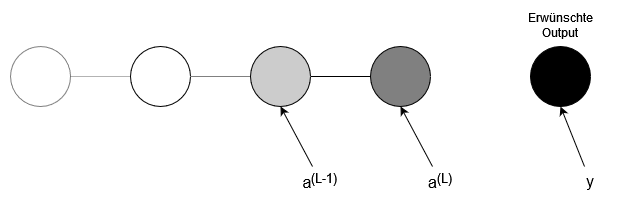
\includegraphics[width=0.75\linewidth]{images/4neurons.png}
	\label{fig:4neurons}
	\caption{4 Neuronen für die Back-Propagation ( Bild von \href{https://www.youtube.com/watch?v=tIeHLnjs5U8}{3Blue1Brown})}
\end{figure}

\[\sigma '(x) = \sigma(x)\; (1-\sigma(x))\]

\noindent Die Funktion ist die Ableitung der Sigmoid-Funktion, die in der neuronalen Netzwerkoptimierung für die Gewichtsaktualisierung mittels Backpropagation verwendet wird.

\[z^{(L)} = w^{(L)}\; a^{(L-1)}+b^{(L)}\]
\[a^{(L)} = \sigma(z^{(l)})\]
\[y = erwartete\; Output\]


\begin{figure}[H]
	\centering
		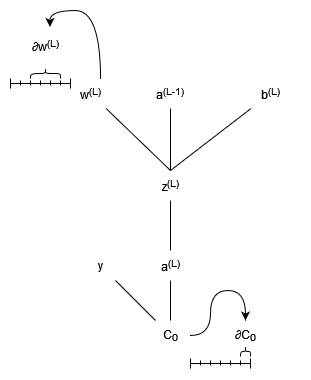
\includegraphics[width=0.5\linewidth]{cost_tree.png}
	\label{fig:cost_tree}
	\caption{Kostenbaum in der Back-Propagation ( Bild von \href{https://www.youtube.com/watch?v=tIeHLnjs5U8}{3Blue1Brown})}
\end{figure}


\[Cost_0(\cdots) = C_0 = (a^{(L)}-y)^2 \]

\noindent Die Formel beschreibt die Kostenfunktion für ein einzelnes Trainingsbeispiel in einem neuronalen Netzwerk. Diese Kostenfunktion, oft als quadratischer Fehler oder Mean Squared Error (MSE) bezeichnet, misst den quadratischen Unterschied zwischen der vorhergesagten Ausgabe und dem tatsächlichen Wert, um die Leistung des Modells zu bewerten und während des Trainingsprozesses zu optimieren.

\[\frac{\partial C_0}{\partial w^{(L)}} = Empfindlichkeit\; der\; Cost-Funktion\; in\; Bezug\; auf\; das\; Gewicht\]


\[\frac{\partial C_0}{\partial w^{(L)}} = \frac{\partial z^{(L)}}{\partial w^{(L)}}\; \frac{\partial a^{(L)}}{\partial z^{(L)}}\; \frac{\partial C_0}{\partial a^{(L)}}\] %Chainrule (Calculus)

\noindent Diese Formel beschreibt die Berechnung des Gradienten der Kostenfunktion $C_0$ bezüglich des Gewichts $w^{(L)}$ in der letzten Schicht LL eines neuronalen Netzes. Sie nutzt die Kettenregel der Differentialrechnung, um den Einfluss von Änderungen im Gewicht auf die Kosten zu ermitteln, indem sie das Produkt aus der Ableitung des Netzeingangs $z^{(L)}$ nach dem Gewicht, der Ableitung der Aktivierungsfunktion $a^{(L)}$ nach dem Netzeingang und der Ableitung der Kostenfunktion nach der Aktivierung berechnet.

\[\frac{\partial C_0}{\partial a^{(L)}} = 2(a^{(L)}-y)\]
\[\frac{\partial a^{(L)}}{\partial z^{(L)}} = \sigma '(z^{(L)}\]
\[\frac{\partial z^{(L)}}{\partial w^{(L)}} = a^{(L-1)}\]
\[\frac{\partial C_0}{\partial w^{(L)}} = a^{(L-1)}\; \sigma '(z^{(L)}\; 2(a^{(L)}-y)\]

\noindent Dies ist eine spezifischere Formulierung, die direkt die Komponenten aus der oberen Gleichung zusammenfasst und annimmt. Diese Gleichungen verbinden also die Änderung des Fehlers in Bezug auf ein Gewicht direkt mit der Aktivierung der vorherigen Schicht.

\[\frac{\partial z^{(L)}}{\partial b^{(L)}} = 1\]
\[\frac{\partial C_0}{\partial b^{(L)}} = 1 \sigma '(z^{(L)}\; 2(a^{(L)}-y)\]

\noindent Diese Funktion berechnet wie die Funktion $\frac{\partial C_0}{\partial w^{(L)}} = a^{(L-1)}\; \sigma '(z^{(L)}\; 2(a^{(L)}-y)$ den Gradienten der Kostenfunktion $C_0$, jedoch nicht in Bezug auf die Gewichtung $w^{(L)}$, sondern auf den Bias $b^{(L)}$.

\[\frac{\partial z^{(L)}}{\partial a^{(L-1)}} = w^{(L)}\]
\[\frac{\partial C_0}{\partial a^{(L-1)}} = w^{(L)}\; \sigma '(z^{(L)}\; 2(a^{(L)}-y)\]

\noindent Diese Formel zeigt, im Gegensatz zu den beiden anderen, wie der Gradient der Kostenfunktion $C_0$ bezüglich der Aktivierungen $a^{(L-1)}$ des vorherigen Layers berechnet wird. So kann diese Funktion, gleich wie die für die Gewichtung und dem Bias, dazu verwendet werden, zu verstehen, wie Änderungen in den Aktivierungen des vorherigen Layers $L-1$ den Gesamtfehler beeinflussen können.

\[\frac{\partial C}{\partial w^{(L)}} = \frac{1}{n}\sum_{k=0}^{n-1} \frac{\partial C_{k}}{\partial w^{(L)}}\]
\[\nabla C = \left(\begin{array}{c} \frac{\partial C}{\partial w^{(1)}} \\ \frac{\partial C}{\partial b^{(1)}} \\ \vdots \\ \frac{\partial C}{\partial w^{(L)}} \\ \frac{\partial C}{\partial b^{(L)}} \end{array}\right)\] %Gradient vector

\noindent Die Gleichung $\frac{\partial C}{\partial w^{(L)}} = \frac{1}{n}\sum_{k=0}^{n-1} \frac{\partial C_{k}}{\partial w^{(L)}}$ beschreibt den Gradienten der Kostenfunktion $C$ in Bezug auf die Gewichte $w^{(L)}$ in der $L$-ten Schicht des Netzwerks. Der Gradient wird als Durchschnitt der Gradienten aus $n$ Trainingsbeispielen berechnet.
\\
\noindent Die 2 Notation ($\nabla C$) stellt den Gradienten der Kostenfunktion $C$ als Vektor dar, der alle partiellen Ableitungen der Kostenfunktion in Bezug auf alle Gewichte $w^{(L)}$ und alle Bias-Werte $b^{(l)}$ für jede Schicht $L$ des Netzwerks enthält. Dieser Gradientenvektor ist wesentlich für die Anwendung des Gradientenabstiegsverfahrens, da er die Richtung angibt, in der die Gewichte und Bias-Werte angepasst werden müssen, um die Kostenfunktion zu minimieren.

\noindent\textbf{Mit mehreren Outputs:}

\begin{figure}[H]
	\centering
		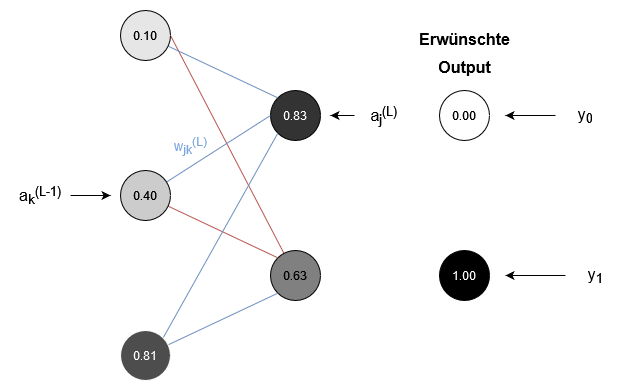
\includegraphics[width=0.75\linewidth]{images/nn5bp.png}
	\label{fig:nn5bp}
	\caption{5 Neuronen in einem Netzwerk ( Bild von \href{https://www.youtube.com/watch?v=tIeHLnjs5U8}{3Blue1Brown})}
\end{figure}

\noindent Dies sind im Grundsatz die gleichen Funktionen wie oben, es wurde ihnen aber eine weitere Komplexitätsstufe hinzugefügt, indem nun das Netzwerk nicht mehr aus nur einem Neuron pro Layer besteht.

\[C_0 = \sum_{j=0}^{n_{L}-1} (a_j^{(L)} - y_j)^2\]
\[z_j^{(L)} = \cdots + w_{jk}^{(L)}\; a_k^{(L-1)} + \cdots + b_j^{(L)}\]
\[a_j^{(L)} = \sigma(z_j^{(L)})\]
\[\frac{\partial C_0}{\partial w_{jk}^{(L)}} = \frac{\partial z_j^{(L)}}{\partial w_{jk}^{(L)}}\; \frac{\partial a_j^{(L)}}{\partial z_j^{(L)}}\; \frac{\partial C_0}{\partial a_j^{(L)}}\]
\[\frac{\partial C_0}{\partial a_k^{(L-1)}} = \sum_{j=0}^{n_{L} - 1} \frac{\partial z_j^{(L)}}{\partial a_k^{(L-1)}}\; \frac{\partial a_j^{(L)}}{\partial z_j^{(L)}}\; \frac{\partial C_0}{\partial a_j^{(L)}}\]

\mbox{}\\\

\[\frac{\partial C}{\partial w_{jk}^{(l)}} = a_k^{(l-1)}\; \sigma '(z_j^{(l)})\; \frac{\partial C}{\partial a_j^{(l)}}\]
\[
\begin{split}
\frac{\partial C}{\partial a_j^{(l)}}\  & = \sum_{j=0}^{n_{l+1}-1} w_{jk}^{(l+1)}\; \sigma '(z_j^{(l+1)})\; \frac{\partial C}{\partial a_j^{(l+1)}}\; \\
&\qquad or \\
& 2(a_j^{(L)}-y_j)
\end{split}
\]